% Carried over verbatim from monograph/main.tex (Study 1 record, 13 Sep 2026).
\chapter{The parent-identity mechanism probe}\label{s1:ch:ch09_the_parent_identity_mechanism_probe}

\section{Motivation}

Structural overlap says that siblings are present. The parent probe asks whether their shared source is visually recoverable after cellular content and color cues are altered. A positive answer makes the shortcut concrete: a learner can recognize the parent field from a different crop. It still does not prove that a morphology classifier uses that signal.

\section{Balanced task construction}

Parents with at least four crops are eligible. The minimum eligible size allows two training and two test crops per parent. To make chance exact, each eligible parent contributes the same number of training and test crops. The final task contains 424 parents, 848 training crops, and 848 test crops, so chance is
\begin{equation}
P_{\mathrm{chance}}=\frac{1}{424}=0.00235849=0.235849\%.
\end{equation}

A ResNet-18~\cite{he2016resnet} initialized from ImageNet replaces its final layer with a 424-way linear classifier. It trains for 15 epochs with AdamW~\cite{loshchilov2019adamw}, learning rate $10^{-4}$, weight decay $10^{-4}$, batch size 64, and fixed seeds. Training augmentation is a random resized crop with scale 0.85--1.0 plus horizontal and vertical flips; testing resizes to $224\times224$. ImageNet normalization follows every image-mode transform.

\section{Image transformations and their motivations}

\subsection{RGB}
RGB is the maximal-information condition. It permits morphology, stain, illumination, background, focus, acquisition artifacts, and any other visible cue.

\subsection{Grayscale}
Grayscale removes hue and saturation while retaining luminance, edges, morphology, focus, and texture. Persistence here means identity is not solely a stain-color phenomenon.

\subsection{LAB stain normalization}
RGB is converted to CIE LAB. For channel vector $z$, source mean $\mu_s$, source standard deviation $\sigma_s$, and fixed target statistics $\mu_t=(190,140,135)$ and $\sigma_t=(35,14,14)$, the implemented transform is
\begin{equation}
z'=\operatorname{clip}\left((z-\mu_s)\odot\frac{\sigma_t}{\max(\sigma_s,1)}+\mu_t,0,255\right).
\end{equation}
This is a fixed-statistics color-transfer normalization based on the logic of Reinhard et al.~\cite{reinhard2001color}. Persistence means simple first- and second-moment color normalization does not erase the source fingerprint.

\subsection{Background-only: Otsu, morphology, and Telea inpainting}

This condition deliberately removes the likely cell foreground. The implementation converts RGB to HSV and grayscale, then independently obtains Otsu thresholds~\cite{otsu1979threshold} on saturation $S$ and luminance $Y$. The preliminary foreground mask is
\begin{equation}
M_0(u)=\mathbf{1}\{S(u)>t_S\;\lor\;Y(u)<t_Y\}.
\end{equation}
A $5\times5$ morphological closing fills small holes and connects narrow gaps:
\begin{equation}
M=(M_0\oplus K)\ominus K.
\end{equation}
Finally, the marked region is filled from its boundary with Telea's fast-marching inpainting method using radius 5~\cite{telea2004inpainting}. The result keeps background statistics while suppressing the cell body and nucleus. A successful classifier in this condition shows that background alone carries considerable parent information.

\subsection{High-pass}
For Gaussian blur $G_{\sigma=3}*I$, the residual is
\begin{equation}
I_{\mathrm{hp}}=\operatorname{clip}\left(I-G_{\sigma=3}*I+128,0,255\right).
\end{equation}
This suppresses low-frequency illumination and emphasizes local texture, edges, compression, and focus structure.

\begin{figure}[H]
\centering
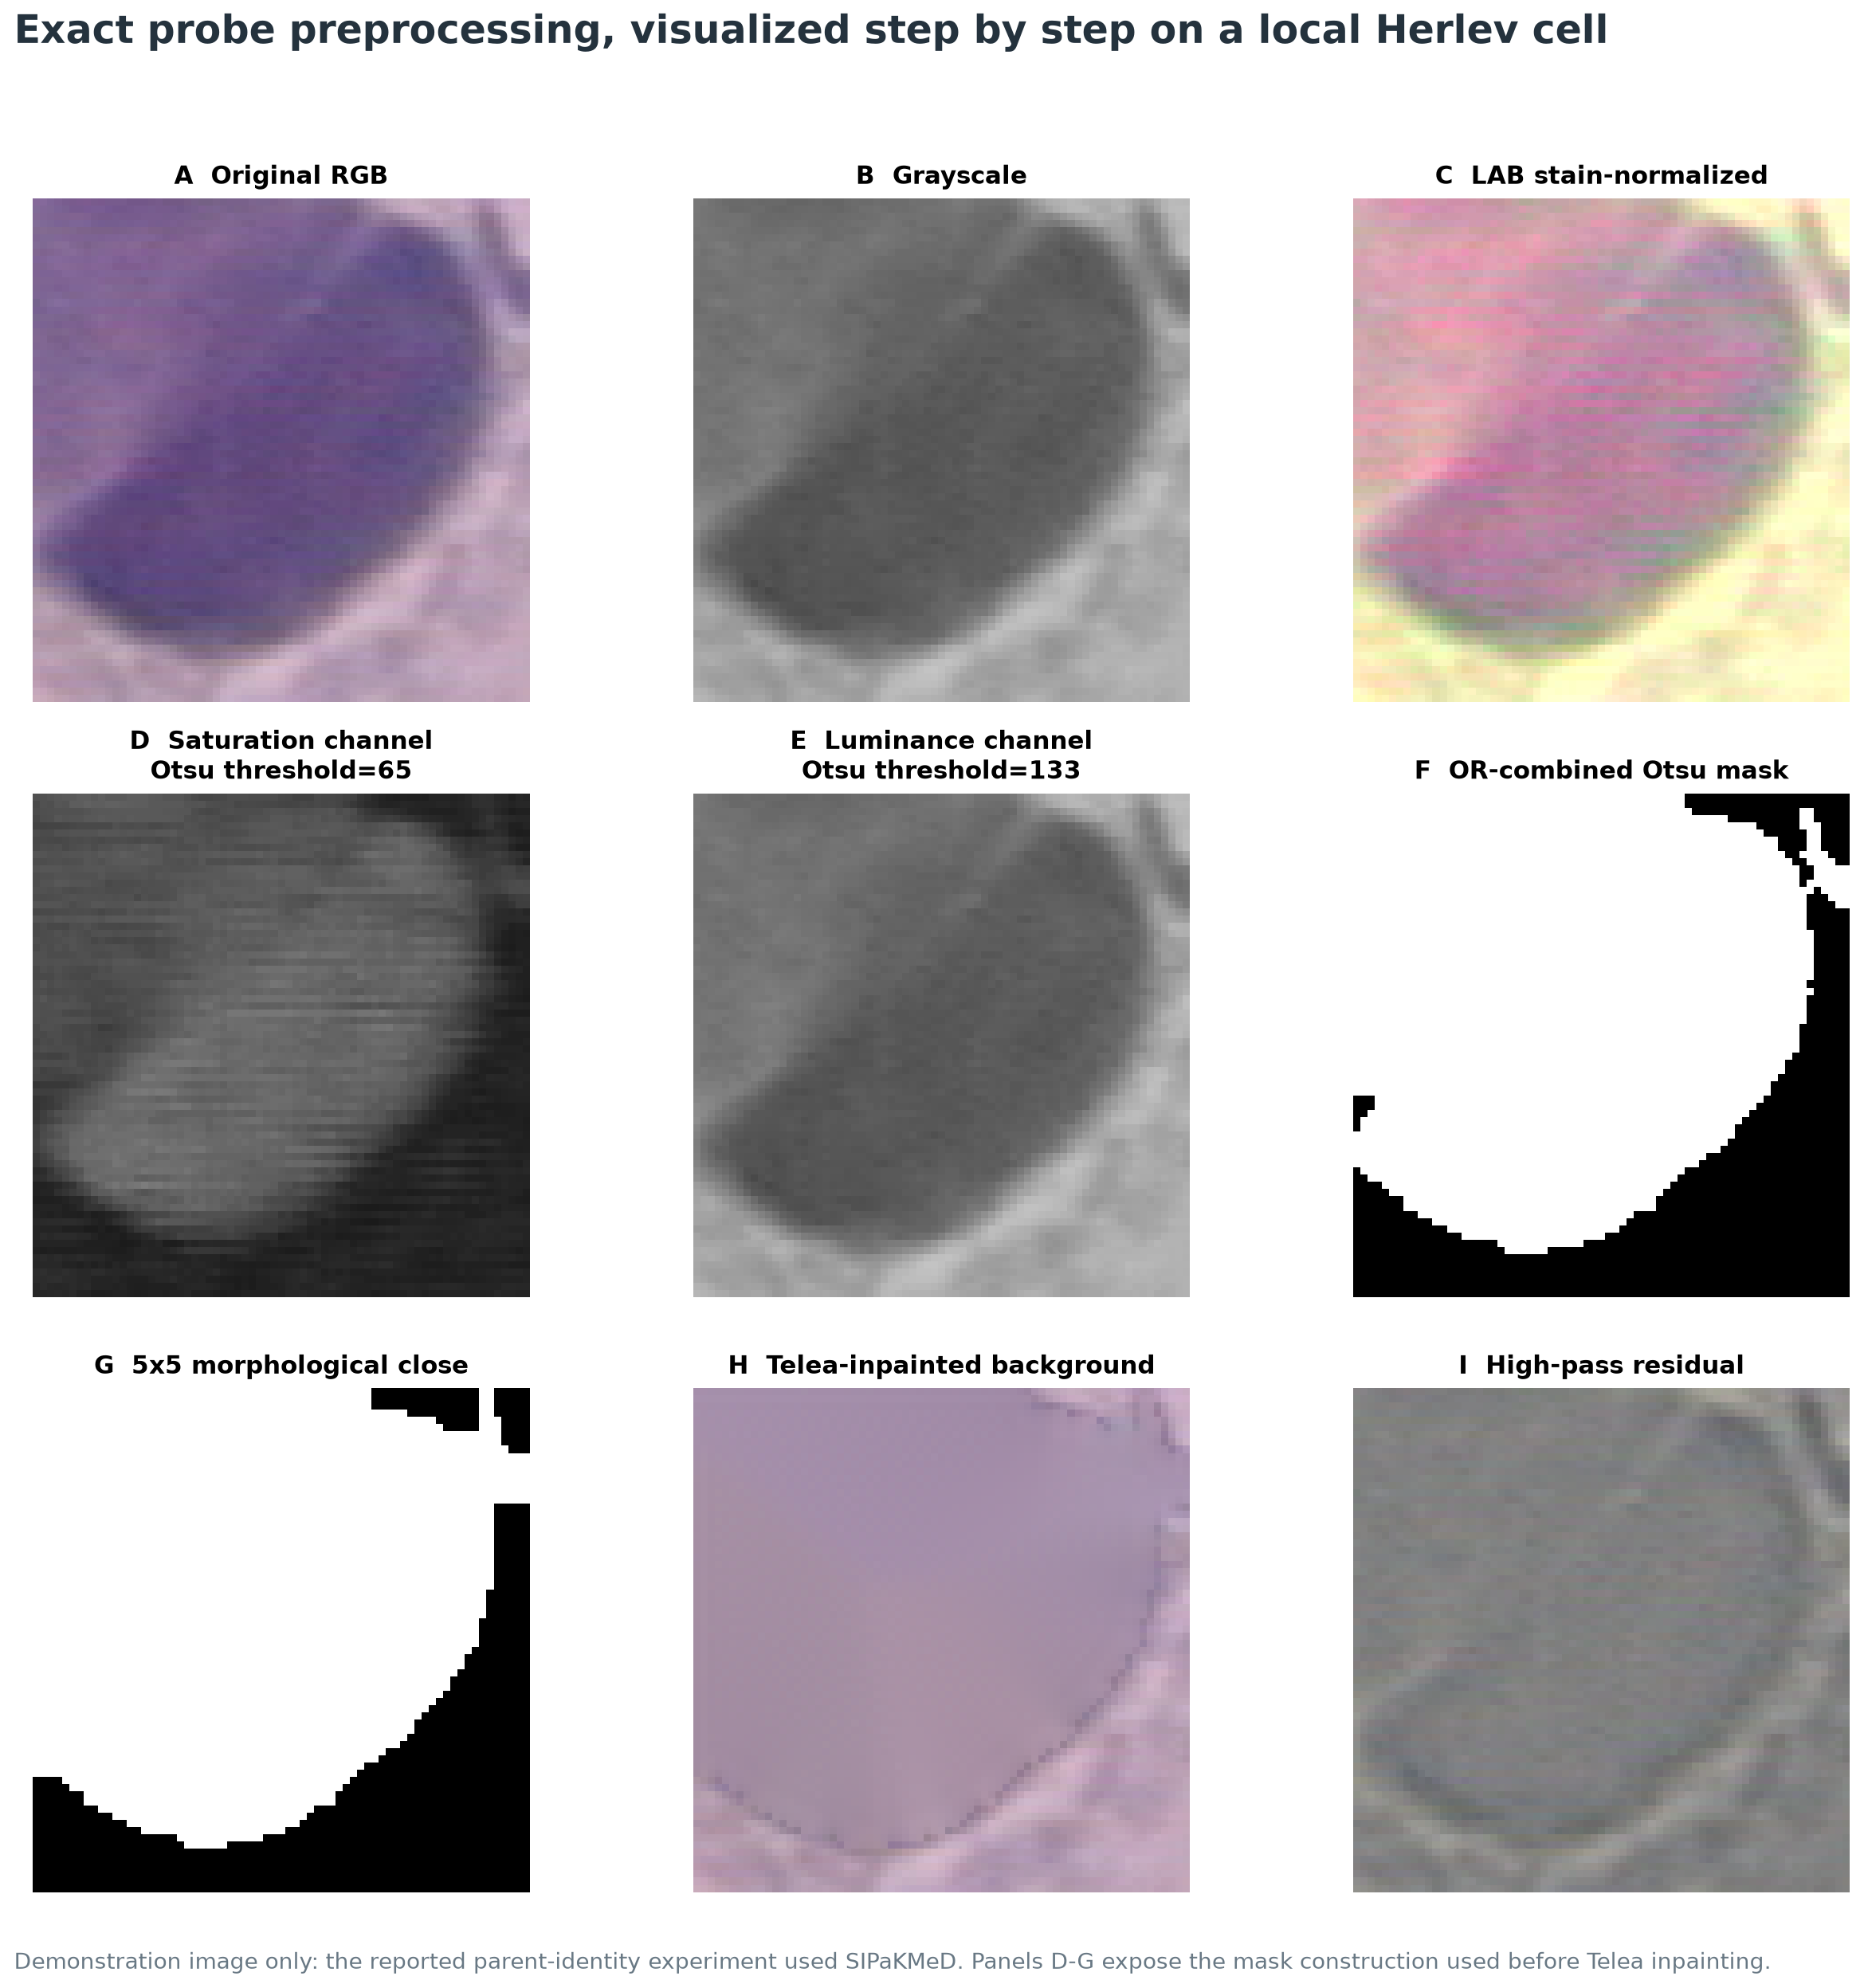
\includegraphics[width=0.92\textwidth]{probe_transformations.png}
\caption{Every preprocessing stage shown on an actual local Herlev cell. This is an implementation demonstration, not a probe result image: the reported parent-identification experiment used SIPaKMeD crops. Panels D--G make Otsu thresholding, mask combination, and morphological closing visible before Telea inpainting.}
\label{s1:fig:transformations}
\end{figure}

\section{Shuffled-label negative control}

Only the training labels are permuted, using the same images, optimizer, epochs, seeds, and task size. The five-seed 95\% interval must cover the exact chance baseline. Otherwise the probe would be rejected because a bookkeeping or imbalance artifact could explain apparent identity learning.

\section{Results}

\begin{table}[H]
\centering
\caption{Parent-identity probe. Mean $\pm$ sample SD over five seeds.}
\label{s1:tab:probe}
\begin{tabular}{lrr}
\toprule
Input condition & Accuracy & Multiple of chance \\
\midrule
RGB & 25.73$\pm$0.66\% & 109.1$\times$ \\
Grayscale & 13.80$\pm$1.12\% & 58.5$\times$ \\
Stain-normalized & 17.31$\pm$0.64\% & 73.4$\times$ \\
Background-only & 18.68$\pm$1.25\% & 79.2$\times$ \\
High-pass & 16.27$\pm$0.60\% & 69.0$\times$ \\
Shuffled RGB labels & 0.17$\pm$0.24\% & 0.7$\times$ \\
\bottomrule
\end{tabular}
\end{table}

\begin{figure}[H]
\centering
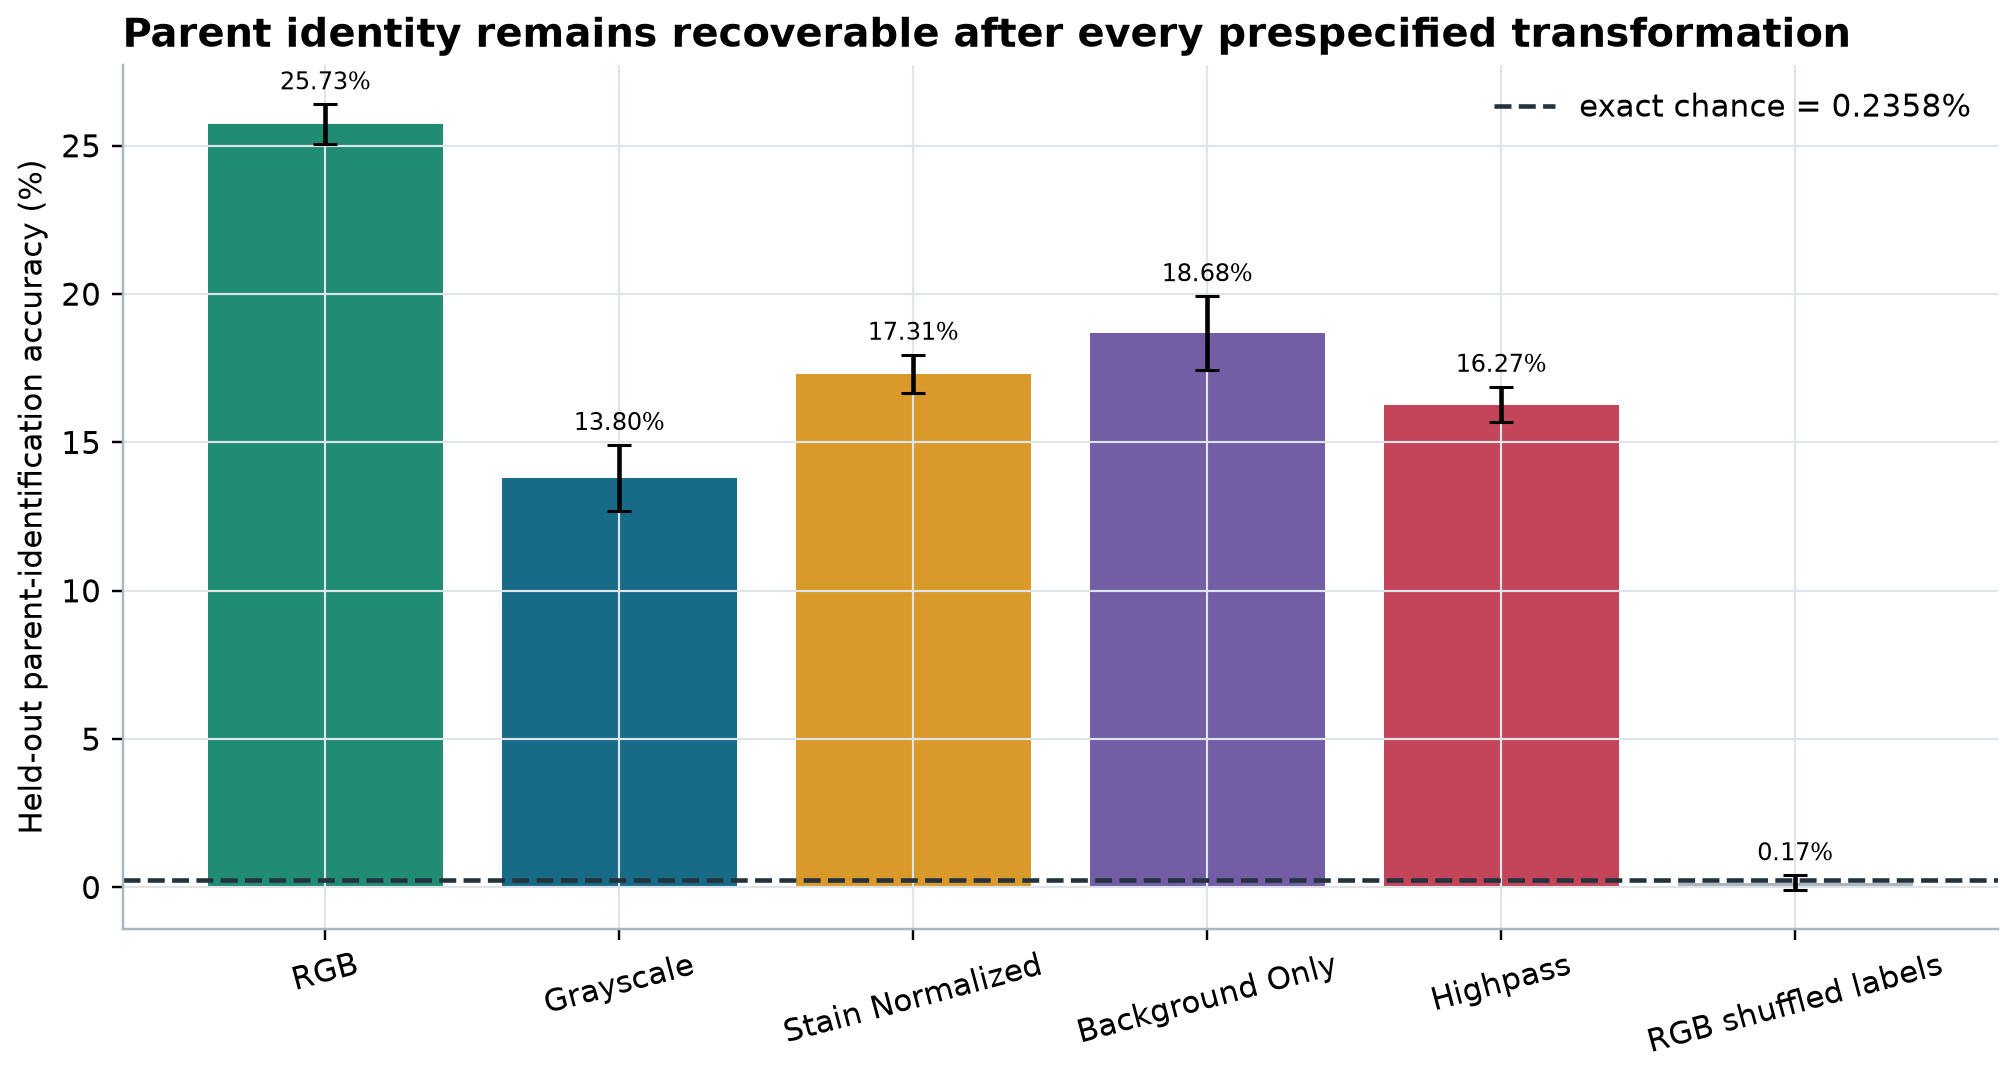
\includegraphics[width=0.92\textwidth]{probe_results.png}
\caption{All prespecified image conditions remain far above chance. Error bars are sample SD across five seeds.}
\label{s1:fig:probe-results}
\end{figure}

\begin{figure}[H]
\centering
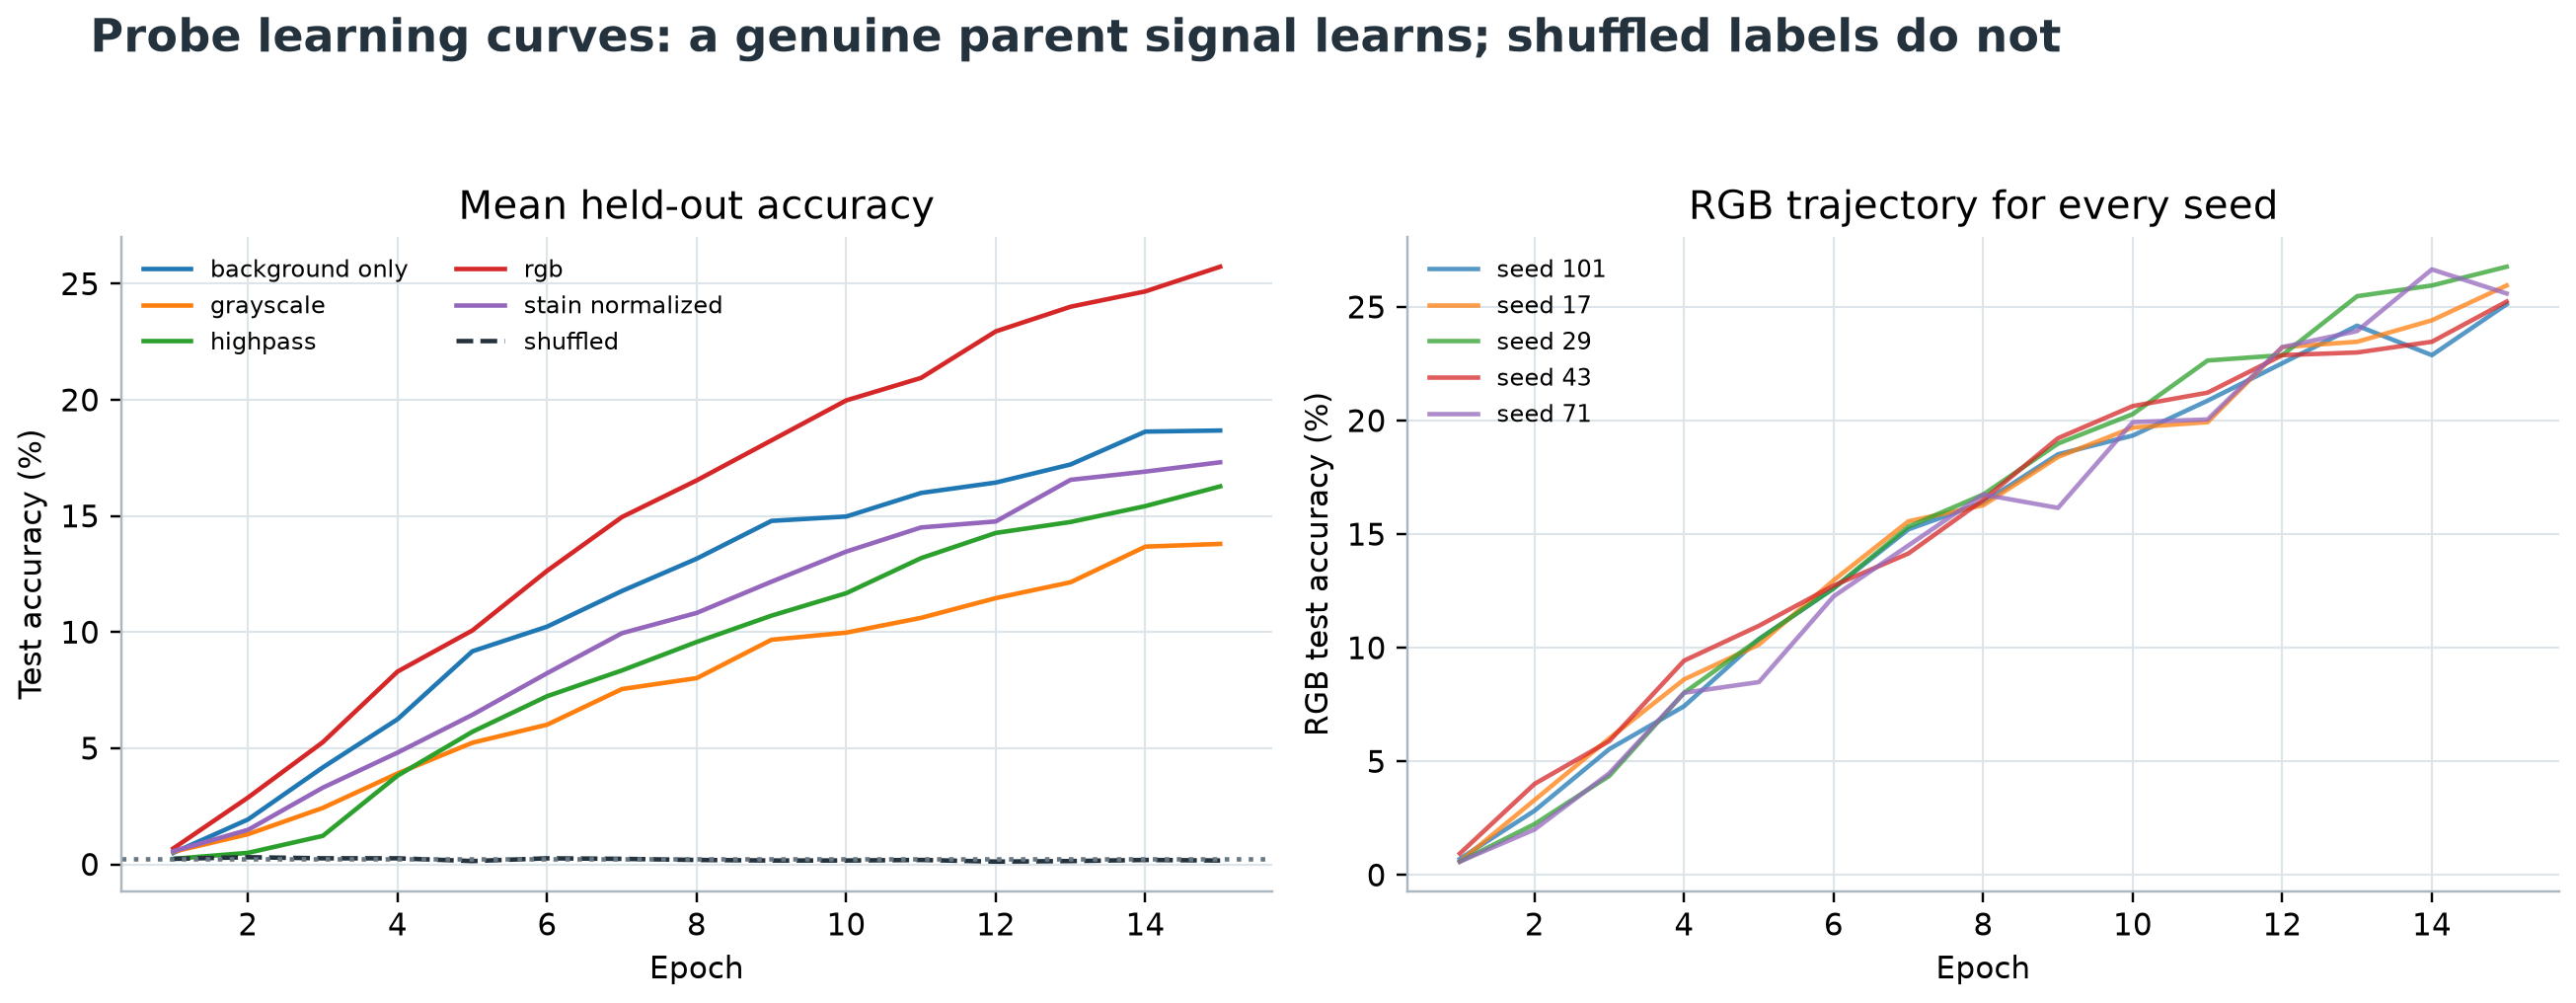
\includegraphics[width=\textwidth]{probe_learning_curves.png}
\caption{Probe learning curves reconstructed from every retained epoch history. The RGB signal rises smoothly across seeds; shuffled labels remain near chance.}
\label{s1:fig:probe-learning}
\end{figure}

The shuffled mean is 0.1651\%, SD 0.2445 percentage points, with a five-seed interval from $-0.1385$\% to 0.4687\%; the exact 0.2358\% chance value lies inside. A negative lower confidence limit is an ordinary symmetric small-sample interval artifact and does not imply negative accuracy.

Background-only accuracy is higher than grayscale and stain-normalized accuracy. That does not mean background is the only cue: RGB remains highest, and transformations alter multiple image properties at once. The careful conclusion is that parent information is distributed across color, low- and high-frequency structure, and background.
